\documentclass[10pt,conference]{IEEEtran}
%\documentclass[conference]{IEEEtran}

\makeatletter
\def\ps@headings{%
\def\@oddhead{\mbox{}\scriptsize\rightmark \hfil \thepage}%
\def\@evenhead{\scriptsize\thepage \hfil \leftmark\mbox{}}%
\def\@oddfoot{}%
\def\@evenfoot{}}
\makeatother

\pagestyle{headings}

\newcommand{\nop}[1]{}
\usepackage{graphicx}
\usepackage{epsfig}
\usepackage{balance}
\usepackage{algorithm}
\usepackage{algorithmic}
\usepackage[centertags]{amsmath}

\newtheorem{definition}{Definition}
\newtheorem{remark}{Remark}

\def\linespaces{0.95}
\def\baselinestretch{\linespaces}


\begin{document}

\title{Scheduling Recurring Tasks in Energy Harvesting Sensors}
\author{David Audet\\daudet@uvic.ca \and Leandro {Collares de Oliveira}\\leco@uvic.ca \and Neil MacMillan\\nrqm@uvic.ca \and Dimitri Marinakis\\dmarinak@kinsolresearch.com \and Kui Wu\\wkui@uvic.ca}

\maketitle


\begin{abstract}

We consider the problem of periodic task scheduling in sensor nodes powered with energy harvesters. In particular, we focus on systems with stochastic energy sources such as solar panels, and we present two energy-aware scheduling algorithms that reduce the likelihood of task violations. Our algorithms, called \emph{Smooth to Average Method (\textsc{STAM})} and \emph{Smooth to Full Utilization (\textsc{STFU})}, are static schedulers that do not require prescience of the incoming energy to operate effectively.
\end{abstract}

\begin{IEEEkeywords} Real-Time Scheduling, Recurring Tasks, Energy Harvester, Sensors
\end{IEEEkeywords}


\section{Introduction}\label{sec:introduction}

A wireless sensor network (\textsc{wsn}) consists of collaborating sensor nodes with capabilities of sensing, computation and communication~\cite{sudevalyam2010energy}. Wireless sensor networks can be deployed for a plethora of purposes such as habitat monitoring~\cite{mainwaring2002wireless}, earthquake detection~\cite{suzuki2007earthquake}, and healthcare~\cite{saadaoui2007architecture}. 

To make deployment easy, wireless sensor networks usually do not rely on existing infrastructure, and sensor nodes are powered by batteries. On the other hand, the lifetime of these embedded devices is limited by the amount of energy that can be stored in the batteries. Furthermore, the number of sensors and their locations might render the activity of replacing nodes' batteries unfeasible or very costly~\cite{moser2007real}. 

To solve the above problem, intensive research has been conducted on energy harvesting as a way to extend the lifetime of wireless sensor networks. Several types of energy such as solar, eolic (wind), vibrational, and thermal among others can be scavenged from the surroundings of a sensor node to replenish its battery~\cite{roundy2004power}. Promising as it may seem, energy harvesting poses new challenges to the scientific community~\cite{lu2010accurate}:

\begin{itemize}
	\item Environmental energy sources behave stochastically, making the accurate predication on incoming energy amount very difficult.
	\item Conventional task scheduling techniques were not designed for energy-limited scenarios and cannot deal properly with the uncertainty in energy availability.
\end{itemize}

It has been pointed out that the traditional scheduling method, Earliest Deadline First (\textsc{edf}), may not work well under energy-limited conditions~\cite{moser2007real}, and as such new algorithms such as the Lazy Scheduling Algorithm (\textsc{lsa}) has been proposed to ``solve" the problem~\cite{moser2007real}. Although it has been theoretically proved that LSA is optimal, it requires a good predication on the incoming energy source to operate well. We find that energy predication is non-trivial, and it is nearly impossible to implement any ``intelligent" learning algorithm for such purpose over tiny sensors due to the limited computational resource. Installing a pre-trained energy predication model does not work either, because such a model depends on where and when the model was built and may not work well when the sensors are deployed in different places and function over a long time period. 

In this paper, we make contributions by proposing two new scheduling techniques, the Smooth to Average Method (\textsc{stam}) and Smooth to Full Utilization (\textsc{stfu}), to handle the energy uncertainty and deadline constraint without relying on any energy predication model\footnote{Although in the later of the paper, we build an energy charging model for solar energy harvesting. This model is \textit{purely} for the purpose of performance comparison and in real implementation such a model is not required.}.
We consider solar energy scavenging through photo-voltaic conversion, as it provides the highest power density of conventional environmental energy harvesting techniques~\cite{raghunathan2005design}. 

%We use a Markov model based on a matrix of transition probabilities for three radiation %intensity states to predict the power provided by the harvesting unit \cite
%{poggi2000stochastic}.

\section{Related Work} \label{sec:related work}

Important early work in real time scheduling by Liu and Layland~\cite{Liu73} presented two classic scheduling algorithms,
rate-monotonic priority assignment and deadline-driven scheduling, and assessed their performance based on processor
utilization. Their work, however, did not consider energy constraints. 
Moser \emph{et al.}~\cite{moser2007real}, in more recent work, described energy-aware \textsc{lsa} scheduling
and proved that it optimally deals with time and energy constraints in a system whose energy storage is replenished
\textit{predictably}. The suitability of this approach under realistic energy harvesting conditions, however, is unclear. 

Research into energy-aware algorithms for sensor nodes is an active area. Kansal \emph{et al.}~\cite{kansal2007power}
presented power management algorithms based on duty-cycling between active and low-power modes of sensor nodes 
with energy harvesting capabilities to achieve perennial operation at a desired performance level. 
Niyato \emph{et al.}~\cite{niyato2007sleep} investigated the impact of sleep and wake-up strategies 
on data communication among solar-powered nodes. These strategies are dependent on battery charge, solar radiation
level and number of packets in the queue. In~\cite{vigorito2007adaptive}, Vigorito \emph{et al.} proposed an adaptive
duty-cycling algorithm that ensures that power supplied to sensor nodes is kept within operational levels in several
energy harvesting scenarios. The
algorithm does not require previous information on the energy source dynamics and presents low computational
demands. In~\cite{moser2007adaptive}, Moser \emph{et al.} presented an adaptive power management
model that can be customized to address different constraints and optimization objectives in energy harvesting systems 
such as tradeoffs between communication and memory usage.


Predicting stochastic energy sources is non-trivial.  
Lu \emph{et al.}~\cite{lu2010accurate} assessed three prediction techniques, regression analysis,
moving average, and exponential smoothing, which meet the requirements imposed by a real-time energy
harvesting embedded system: high accuracy and low computation and memory demands. 
Recas~\emph{et al.}~\cite{recas2000hollows} employed the Weather-Conditioned Moving Average (\textsc{wcma}) model,
which adapts to seasonal changes in solar power harvesting as well as sudden weather changes. 
Moser \emph{et al.}~\cite{moser2007real} introduced energy variability curves to predict the power provided by a 
harvesting unit. Energy predictions based on these curves are highly accurate when sensor nodes utilization is low.
In~\cite{susu2008stochastic} Susu \emph{et al.} used a discrete-time Markov chain in which only transitions between 
consecutive states, representing energy levels generated by a solar panel, were allowed. This restriction hinges
on the fact that abrupt changes in the energy provided in a time step are highly improbable. 
On the other hand, Niyato \emph{et al.}~\cite{niyato2007sleep} made use of a Markov chain model that takes into
consideration the influence of clouds and wind on solar radiation intensity. 
Due to the limited computational and memory resources available on a typical sensor node, however,
implementing suitably accurate dynamic energy predication models appears challenging, making 
scheduling algorithms based on energy predication impractical. 

%The majority of energy harvesting systems are based on rechargeable batteries, as noted by Sudevalayam and Kulkarni~\cite{sudevalyam2010energy}.
%However, Simjee and Chou~\cite{simjee2007everlast} add that there has been increasing interest in %supercapacitors, which theoretically have infinite charge cycles and high power densities. 
In~\cite{jiang2005perpetual}, Jiang \emph{et. al.} present a hybrid implementation based on two supercapacitors and one rechargeable battery.



\section{Model and Problem Formulation} \label{sec:model}

To model task execution in the sensor nodes, we assume the following: 
\begin{itemize}
	\item (A1) The requests for all tasks are periodic, with constant interval between requests. 
	\item (A2) Each request of a task has a hard deadline, which is defined as the time when the next request for the task arrives. 
	\item (A3) A task has constant run-time. Run-time refers to the time that  is taken by the microprocessor to execute the task without interruption.
	\item (A4) The task drains energy with a constant rate during its execution time\footnote{Energy consumption on sensor nodes largely depends on the operations of peripheral devices (e.g., sensors and wireless transmitters) associated with the task rather than executing code in the microprocessor.}.       
	\item (A5) The tasks are independent in that requests for a given task do not depend on the initialization or the completion of requests for other tasks.
	\item (A6) A schedule exists that satisfies the timing requirements of all tasks.
\end{itemize}

To model the energy harvester component we assume the following:
 \begin{itemize}
	\item (A7) The energy harvester provides energy source to the node with a power function $P_S(t)$, which can be modeled as a stationary random process during the time in consideration.
	\item (A8) The sensor node also includes an energy storage module (capacitors or rechargeable batteries) with the maximum capacity of $C$. 
\end{itemize}
 
We can denote a set of recurring tasks by $\{\tau_1, \tau_2, \ldots, \tau_n\}$, with each task represented by a tuple $\tau_i = <I_i, T_i, E_i>$, where $I_i$ denotes the periodic interval time between requests for the task, $T_i$ denotes the task's execution time, and $E_i$ denotes the task's energy consumption. We denote the harvester component by $<C(t), P_S(t)>$, where $C(t)$ is the energy capacity at time $t$ and $P_S(t)$ is the stochastic energy input function. For a set of tasks scheduled according to some scheduling algorithm, we say that a \textit{violation} occurs at time $t$ if the node's energy level drops to zero.

In this paper we consider the question of how best to schedule tasks to reduce the likelihood of causing an energy violation.


\section{New Energy-Aware Scheduling Algorithms} \label{sec:algorithms}
We have developed two new techniques that, when combined with known scheduling algorithms, reduce the likelihood of an energy violation while meeting task deadlines.  We call the algorithms the \emph{Smooth to Average Method} (\textsc{STAM}) and \emph{Smooth to Full Utilization} (\textsc{STFU}).

\subsection{Smooth to Average Method}
First we illustrate a core concept, \emph{virtual tasks}, used in our methods.

\begin{definition}
Given a task $\tau_i = <T_i, D_i, E_i>$ and an energy threshold value $\bar{E}$, its equivalent \emph{virtual task} is defined as the task $\bar{\tau}_i = <T_i, \bar{D}_i, \bar{E}_i>$.  For \textsc{STAM}, $\bar{D}_i = \lceil D_i \times  E_i / \bar{E} \rceil$ and $\bar{E}_i = D_i \times  E_i / \bar{D}_i$.
\end{definition}

To distinguish, we call the real task $\tau_i$ a \emph{physical task} in the rest of the paper.

\begin{remark}
When the energy threshold value $\bar{E}$ is larger than $E_i$, the task $\tau_i$ is the same as the task $\bar{\tau}_i$. When the energy threshold value $\bar{E}$ is smaller than $E_i$, task $\tau_i$ and the virtual task $\bar{\tau}_i$ will consume the same amount of energy, spread over a longer execution time than task $\tau_i$.  Any scheduling algorithm that can schedule the virtual task without violating its deadline constraint will meet the deadline for the physical task as well. %point out no voltage scaling needed? - nrqm
\end{remark}
\begin{remark}
The motivation of introducing virtual tasks is to smooth the energy consumption in the long run. If we make a schedule using the virtual tasks, but actually execute the physical tasks according to the schedule, the consequence is that the system will automatically wait for energy replenishment before running a request that consumes a large amount of energy. The waiting time is proportional to the energy amount consumed by the request.
\end{remark}

Intuitively, it would be a good choice to smooth the energy consumption to the average energy requirement per unit time of all tasks in a given task list. The \textsc{STAM} is designed for such a purpose. We generate a set of equivalent \emph{virtual tasks} by increasing the duration of any task that uses greater than average energy per unit time, thus \emph{smoothing} each task to approximately the average energy per time unit. In these virtual tasks, the total energy remains the same as that in the real tasks.  Virtual tasks cannot be scheduled to run at the same time and are not preemptible.  Once the virtual tasks are scheduled, the physical tasks are inserted at the end of the corresponding virtual task's timeslot.  Thus a physical task that consumes high energy is guaranteed to run after an idle period during which energy is harvested, and so the likelihood decreases that the system will run out of energy when the task runs. 

\begin{algorithm}[htb]
\label{stamalg}
\begin{algorithmic}
\STATE INPUT: $realTasks$ \COMMENT {list of [period, duration, energy]} 
\STATE INPUT: $N$ \COMMENT {number of tasks}
\STATE OUTPUT: $vTasks$ \COMMENT {same format as $realTasks$}
\STATE $\bar{E} \gets mean(realTasks[:,3])$
\FOR{$i = 1$ \TO $N$}
\IF{$taskList[i,3] > \bar{E}$}
\STATE $E_{tot} \gets realTasks[i, 2] \times realTasks[i,3]$
\STATE $\bar{D} \gets \lceil E_{tot} / \bar{E} \rceil$
\STATE $\bar{E} \gets \frac{E_{tot}}{\bar{D}}$
\STATE $vTasks[i,:] \gets [taskList[i,1]~~\bar{D}~~\bar{E}]$
\ELSE
\STATE $vTasks[i,:] \gets taskList[i,:]$
\ENDIF
\ENDFOR
\end{algorithmic}
\caption{Generate \textsc{STAM} Task List}
\end{algorithm}

The \textsc{STAM} algorithm calculates the energy consumption of each task by multiplying its runtime by the task's energy consumption per time unit. After taking the mean energy consumption across all of the tasks in the task list, each task is compared to the this value and virtual tasks are generated accordingly. If the given task's energy consumption is above the mean energy value, the virtual duration is calculated by taking the ceiling of the energy area of the task divided by the calculated energy mean. This will extend the duration of the virtual task allowing the total energy consumed to be more evenly distributed across the duration of the task's runtime. If the given task's energy consumption is below the calculated energy mean, the algorithm is unable to perform any smoothing and  will use the unchanged physical task to generate a schedule.

\subsection{Smooth to Full Utilization}

A potential problem of \textsc{STAM} is that the virtual tasks may be spread across too long a duration such that no scheduling is possible to meet the deadline constraints of the virtual tasks. This may happen if some physical tasks require very high energy amount and thus the corresponding virtual tasks enforce the system to wait for a long time. To avoid this problem, we propose a different heuristic to smooth the energy consumption, called \emph{Smooth to Full Utilization} (\textsc{STFU}).  A \emph{virtual task} generated by \textsc{STFU} is defined as the task $\bar{\tau}_i = <T_i, \bar{D}_i, \bar{E}_i>$ where $\bar{D}_i = \lceil D_i \times  E_i / \bar{E} \rceil$ and $\bar{E}_i = D_i \times  E_i / \bar{D}_i$.

The \textsc{STFU} algorithm is similar to \textsc{STAM}, but instead of smoothing all tasks to the average energy usage, \textsc{STFU} attempts to create a virtual task list with 100\% \emph{virtual utilization}\footnote{The CPU utilization calculated based on virtual tasks is called virtual utilization.}, $U_V$.  In other words, in a schedule generated from a virtual task list output by \textsc{STFU}, the likelihood of there being a virtual task scheduled at any arbitrary time is as close as possible to 100\%.

Utilization $U$ is defined in equation~\ref{eqn:utilization}, where $k$ is the number of tasks, $D_i$ is the duration of the $i^{th}$ task, and $T_i$ is the period of the $i^{th}$ task.
\begin{equation}
\label{eqn:utilization}
U = \sum_{i=1}^{k} \frac{D_i}{T_i}
\end{equation}

To generate a virtual task list with \textsc{STFU}, first each task is given a virtual duty cycle $d_V$ representing what proportion of the total run time will be allocated to the corresponding virtual task.  The goal of \textsc{STFU} is to allocate more time to tasks that use greater energy, so that a high-energy task has more time to harvest energy before executing.  A task that uses $40\%$ of the total energy consumed by tasks should be given a virtual duty cycle of $d_V=40\%$.  Virtual tasks cannot have a shorter duration than their real equivalents (otherwise the real task would not fit in the virtual task's timeslice), so if a task's physical duty cycle $d$ is greater than $d_V$ then it will be unchanged.

\begin{algorithm}[htb]
\label{alg:stfualg}
\begin{algorithmic}
\STATE INPUT: $realTasks$ \COMMENT {list of $\bar{\tau}_i = <T_i, D_i, E_i>$} 
\STATE INPUT: $N$ \COMMENT {number of tasks}
\STATE OUTPUT: $vTasks$ \COMMENT {same format as $realTasks$}
\STATE $E_{total} = 0$
\FOR{$i = 1$ \TO $N$}
\STATE $d_i \gets D_i / T_i$
\STATE $E_i^* \gets d_i \times E_i$
\STATE $E_{total} \gets E_{total} + E_i^*$
\ENDFOR
\FOR{$i = 1$ \TO $N$}
\STATE $d \gets E_i^* / E_{total}$
\STATE $d_{V} \gets max(D_i, \left \lfloor T_i \times d \right \rfloor)$
\STATE $E_V \gets D_i \times E_i / d_{V}$
\STATE $vTasks[i] \gets [T_i~~d_{V}~~E_V]$
\ENDFOR
\end{algorithmic}
\caption{Generate \textsc{STFU} Task List}
\end{algorithm}

Figure~\ref{fig:edftasksched}, Figure~\ref{fig:stamtaskplot}, and Figure~\ref{fig:stfutaskplot} show four tasks scheduled by EDF, ALAP with \textsc{STAM}, and EDF with \textsc{STFU}, respectively.  Like in \textsc{STAM}, each real task with \textsc{STFU} smoothing is scheduled at the end of its virtual equivalent's time slice.  The third task, which uses the most energy over a long run, is scheduled after a long period spent collecting energy.  The second task uses very little energy overall, and is given just a short period to collect energy.  For this task set, $U \approx 27\%$ and $U_V \approx 96\%$.


\begin{figure}[htb]
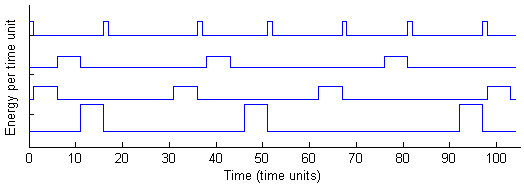
\includegraphics[scale=0.64]{edftasks.png}
\label{fig:edftasksched}
\caption{Four tasks scheduled by EDF with no smoothing.}
\end{figure}

\begin{figure}[htb]
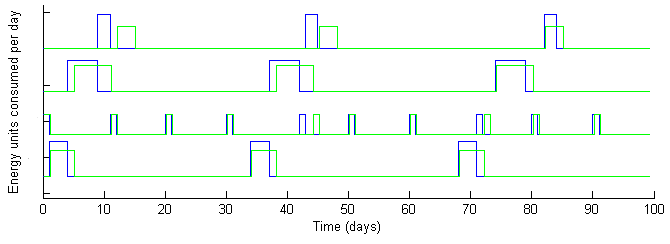
\includegraphics[scale=0.64]{stamtasks.png}
\caption{Four tasks scheduled by EDF with \textsc{STAM} smoothing}
\label{fig:stamtaskplot}
\end{figure}


\begin{figure}[htb]
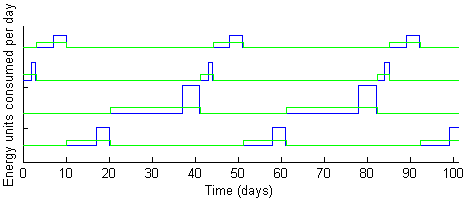
\includegraphics[scale=0.64]{stfutasks.png}
\caption{Four tasks scheduled by EDF with \textsc{STFU} smoothing}
\label{fig:stfutaskplot}
\end{figure}





































\section{Simulation Evaluation} \label{sec:simulation}

We have developed a simulation framework for comparing schedules generated from \textsc{STAM} and \textsc{STFU} task lists to schedules generated from non-smoothed task lists.  Our simulation includes a stochastic energy harvesting process, a random task list and \textsc{STAM}/\textsc{STFU} task list generator, the scheduling processes, and an execution process.  We execute $n$ simulations on one task list per run, and generate task lists for $r$ runs.  Each task list consists of $k$ tasks.

\subsection{Task Generation}
The tasks are generated with random periods, durations, and energy requirements.  The periods and durations are distributed uniformly in discrete time steps measured in days, ranging respectively from 10 to 40 and from 1 to 4.  The energy is half-normally distributed, and proportional to the task's period (\emph{i.e.} a task requiring high energy is expected to run at a low frequency).

A random task list and its corresponding virtual task list generated by \textsc{STAM} and \textsc{STFU} are generated reiteratively until both lists are temporally schedulable.  We consider a task list temporally schedulable when its CPU utilization $U$ (from equation \ref{eqn:utilization} is less than 100\%.  We assume that the physical task list has less than 50% utilization, to better demonstrate our work.

\subsection{Energy Harvesting Model}
We use a simple model of a photovoltaic energy harvester, which converts solar irradiance $G$ into a current $I_c$, as a stochastic energy source for our simulation.  The energy withdrawn from the environment is modeled as a 3-state Markov chain (\cite{poggi2000stochastic,moser2007real}) representing three weather conditions (figure~\ref{fig:markov}).  At each discrete time step during the simulation the Markov chain is updated, and the energy generated added to an energy pool (\emph{i.e.} a battery).
\begin{figure}[htb]
\begin{center}
\label{fig:markov}
\caption{Markov Chain Weather Model.}
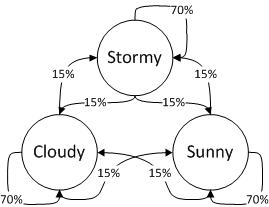
\includegraphics[scale=0.8]{markov.png}
\end{center}
\end{figure}
We generated a table of energy inputs to the system using the solar cell model that comes with Simulink's SimElectronics toolkit, configured with values from \cite{gonzalez2006model}.  
\begin{table}[h]
\begin{center}
\begin{tabular}{| l | l || l | l |}
\hline
\textbf{$G$ ($\frac{W}{m^2}$)} & \textbf{$I_c$ ($A$)} & \textbf{$G$ ($\frac{W}{m^2}$)} & \textbf{$I_c$ ($A$)} \\
\hline
\textbf{50} & \textbf{0.190} & 175 & 0.665 \\
75 & 0.285 & \textbf{200} & \textbf{0.760} \\
\textbf{100} & \textbf{0.380} & 225 & 0.855 \\
125 & 0.475 & 250 & 0.950 \\
150 & 0.570 & 275 & 1.045 \\
\hline
\end{tabular}
\end{center}
\label{tab:radiance}
\caption{Solar panel energy output (bold values are used in our weather model)}
\end{table}
The solar cell's current output with a battery load is related to its radiation input by the linear function $I_c = 0.0038G$.  We use the values of $G = 50, 100, 200 \frac{W}{m^2}$ to represent the stormy, cloudy, and sunny weather conditions in our weather model.

The output current of the photovoltaic cell, $I_c$, is governed by a two-diode formula given in \cite{marwali1997probabilistic} and modeled by the Simulink model.  The current flows into a battery, for which we use a linear model without relaxation effect.  The battery capacity at time $t$, $B_t$ is calculated using equation~\ref{eqn:batterycharge} per \cite{niyato2007sleep}.
\begin{equation}
 B_t = B_{t-1} + I_c \Delta t - I_d \Delta t
\label{eqn:batterycharge}
\end{equation}
where 
\begin{description}
\item[$B_{t-1}$] is the previous battery capacity
\item[$I_c$] is the charge current due to solar harvesting during $\Delta t$
\item[$I_d$] is the discharge current due to task execution during $\Delta t$
\end{description}
We represent $I_c$ and $I_d$  as constant averages during the interval $\Delta t$. Furthermore, the battery is
limited in capacity, such that if $B_t = B_{max}$ then any excess energy that is harvested is lost.

\subsection{Simulation Results}
We performed 1000 runs, with one run consisting of 100 simulations each on several task schedules using common random numbers (\emph{i.e.} using the same weather patterns).  Each simulation covered a period of 100 time units, and if the battery charge dropped to 0 during the simulation we incremented a violation counter.  We recorded the number of violations produced during each run.  

Figure \ref{fig:violations_vs_cpuutil} shows the average number of violations that each algorithm we tried produced over 100 simulations, as a function of physical task utilization.

We used earliest-deadline-first (\textsc{EDF}) and as-late-as-possible (\textsc{ALAP}) scheduling to schedule real tasks, \textsc{STAM} virtual tasks, and \textsc{STFU} virtual tasks (\textsc{STFU} only applies to \textsc{EDF} since high-utilization task lists are hard to schedule with the other algorithms).  In \textsc{EDF}, each task is scheduled as early as possible, in order of increasing deadline.  In \textsc{ALAP}, tasks are scheduled at the latest time possible such that no task misses its deadline.  \textsc{ALAP} is an energy-ignorant version of \textsc{LSA}, which means that it can be scheduled statically without a sophisticated energy prediction model.  

In table \ref{tab:simresults} we show simulation results for statically scheduled systems, and for systems that support dynamic re-scheduling.  The static simulation routine executes each task as it appears in the input schedule.  The dynamic simulator monitors the battery's energy level and, if the battery is at its maximum capacity (\emph{i.e.} harvested energy cannot be stored), tries to re-schedule a task to run immediately.  Our focus in this paper is on static scheduling, but we present results for dynamic scheduling as well.

Our version of \textsc{LSA} is based on the \textsc{LSA-I} algorithm proposed by Moser \emph{et al.} \cite{moser2007real}.  Their work focuses on dynamic scheduling with energy prediction, but we include results for \textsc{LSA-I} for comparison\footnote{Their description of \textsc{LSA-II} is very similar to our implementation of dynamically scheduled \textsc{LSA}, but theirs is further refined via the energy input prediction.}.  To create a static \textsc{LSA} schedule we pre-process an \textsc{ALAP} schedule using our dynamic simulation routine, with a constant minimal energy input in place of the stochastic input.  This constant input is the prediction we give to \textsc{LSA}.  As a result, in \textsc{LSA} tasks will be statically rescheduled when the model can guarantee that the battery is at maximum capacity, \emph{e.g.} at the start of the simulation before any tasks have run.  Energy may still be wasted in the static-schedule, stochastic simulation model when the battery reaches its maximum capacity unexpectedly.  The only way to avoid that would be to predict the energy input while generating the static schedule.
\begin{figure}[htb]
\begin{center}
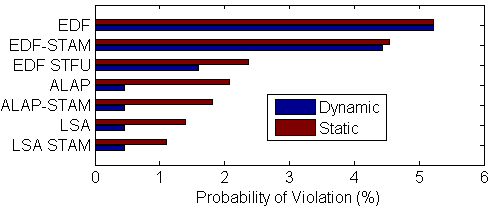
\includegraphics[scale=0.65]{bar.png}
\end{center}
\label{fig:simresults}
\caption{Violations rate for various algorithms with and without dynamic task rescheduling.}
\end{figure}
Figure~\ref{fig:simresults} shows the simulation results for the scheduling algorithms we tested.  As expected, \textsc{EDF}---the optimal periodic scheduling algorithm in systems with unlimited energy---results in the most violations.  Schedules generated by applying the \textsc{EDF} scheduler to the virtual task lists generated by the \textsc{STAM} and \textsc{STFU} algorithms perform better.  Scheduling \textsc{STFU} virtual tasks using \textsc{EDF} results in a significant improvement over plain \textsc{EDF}, approaching the performance of the more complex scheduling algorithms.

The \textsc{ALAP} and \textsc{LSA} static schedulers performed much better than the \textsc{EDF}-based algorithms.  Task lists with high utilization are difficult to schedule with \textsc{ALAP}, so we did not schedule \textsc{STFU} virtual tasks with \textsc{ALAP}.  Using \textsc{STAM} virtual tasks to generate \textsc{ALAP} and \textsc{LSA} schedules improves the results even more.

In the dynamic simulator, \textsc{ALAP} and \textsc{LSA} perform equally well, since our version of \textsc{LSA} is equivalent to \textsc{ALAP} pre-processed with the dynamic simulator.  The dynamic simulations result is a very low violation rate because the model can detect and respond when the battery reaches full capacity unexpectedly.  Running \textsc{ALAP} and \textsc{LSA} on \textsc{STAM} tasks produces slightly worse results than on physical tasks.  This is a result of the small idle time inserted before the physical tasks, which causes energy to be wasted when a \textsc{STAM} task is rescheduled.

\begin{figure}[tb]
\begin{center}
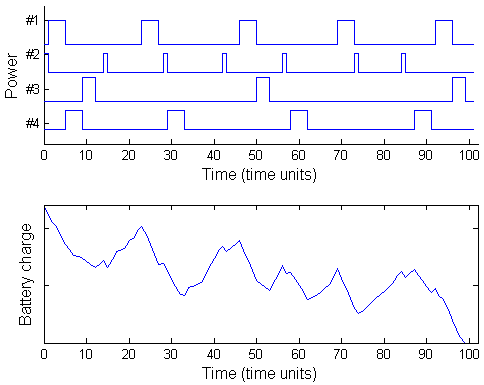
\includegraphics[scale=0.57]{edfbattery.png}
\label{fig:edfbattery}
\caption{Schedule (top) and battery charge level (bottom) during simulation of EDF algorithm.}
\end{center}
\end{figure}

\begin{figure}[tb]
\begin{center}
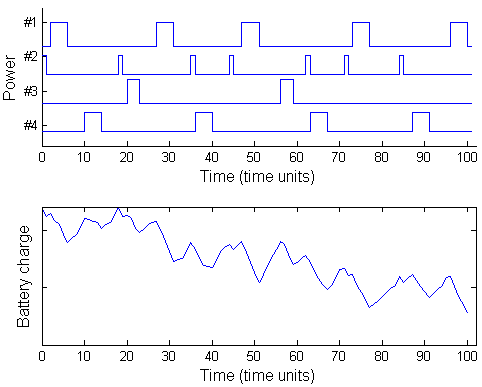
\includegraphics[scale=0.57]{edfstfubattery.png}
\label{fig:edfstfubattery}
\caption{Schedule (top) and battery charge level (bottom) during simulation of EDF algorithm on STFU tasks.}
\end{center}
\end{figure}

\begin{figure}[tb]
\begin{center}
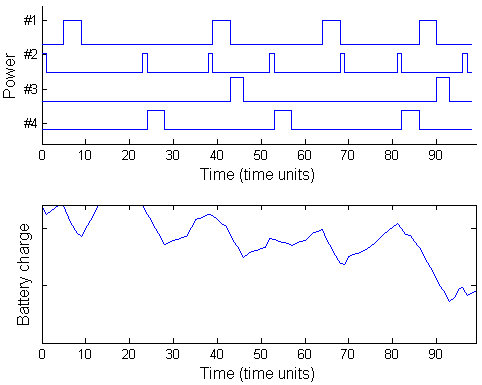
\includegraphics[scale=0.57]{lsabattery.png}
\label{fig:lsabattery}
\caption{Schedule (top) and battery charge level (bottom) during simulation of static LSA algorithm.}
\end{center}
\end{figure}

\begin{figure}[tb]
\begin{center}
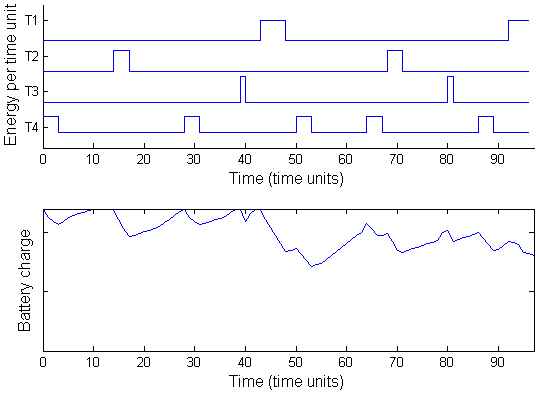
\includegraphics[scale=0.57]{lsastambattery.png}
\label{fig:lsastambattery}
\caption{Schedule (top) and battery charge level (bottom) during simulation of static LSA algorithm with STAM tasks.}
\end{center}
\end{figure}

\begin{figure}[tb]
\begin{center}
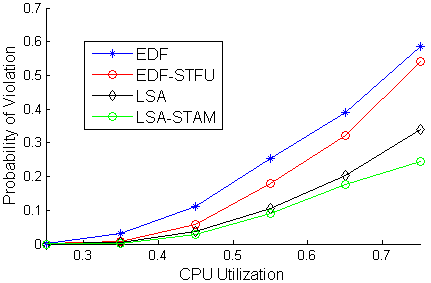
\includegraphics[scale=0.57]{violations_vs_cpuutil.png}
\label{fig:violations_vs_cpuutil}
\caption{Comparison of violation rates}
\end{center}
\end{figure}

Figures \ref{fig:edfbattery} to \ref{fig:lsastambattery} show the change in battery charge level when simulating a particular task list scheduled with four different algorithms with common random numbers.  Figures \ref{fig:edfbattery} and \ref{fig:edfstfubattery} show the relative performance of plain \textsc{EDF} and \textsc{EDF} performed on \textsc{STFU} tasks.  The battery levels for the two simulations are both trending downward at approximately the same rate, but for the \textsc{STFU} simulation the battery level rate of change is smoother.  The large dip in charge that causes a violation at time 99 is ``filtered out'' by \textsc{STFU}, which gives the system a chance to collect more power and recover.  The smoothing effect is also demonstrated in figures \ref{fig:lsabattery} and \ref{fig:lsastambattery} for the static \textsc{LSA} algorithm with and without \textsc{STAM}.


































\section{Conclusion} \label{sec:conclusion}




%\balance




\bibliographystyle{abbrv}

\bibliographystyle{plain}
%\small \baselineskip 9pt
\bibliography{referenceEnergy}

\end{document}
